

\documentclass[main]{subfiles}

\begin{document}


\chapter{Methodology}

\section{Overview}

A panel of four local attribution methods were chosen for evaluation in this project, picked for representativeness of approach and their prominence in the literature. The panel was also a balanced selection from both `classes' of method approach: model-specific (Section \ref{sec:modelspec}) and model-agnostic (Section \ref{sec:modelag}):

\begin{enumerate}

\item \textbf{DeepLIFT:} Model-specific class, backpropagation-based approach (\ref{sec:backprop})
\item \textbf{GradCAM:} Model-specific class, gradient-based approach (\ref{sec:gradient})
\item \textbf{LIME:} Model-agnostic class, perturbation-based approach (\ref{sec:perturbag})
\item \textbf{SHAP:} Model-agnostic class\footnote{Due to its higher level formulation, SHAP has to be implemented for each model family. It's therefore better described as \textit{partially} model-agnostic.}, generic approach (\ref{sec:othermodelag})

\end{enumerate}

Other methods could have been included in this panel though as related work has shown in \ref{sec:existing_studies} (particularly by Ancona et al. (2017)), similarities in formulation should allow conclusions on one method to apply to close relatives. Project constraints also meant that a decision on the panel breadth had to be made according to at least some criteria, and representativeness helps for comparing approaches (the main project goal).

This chapter is presented in sequential order of project milestones, from initial data collection through to fine-tuning of the evaluation metrics designed. The evaluation methodology itself can be summarised in terms of the dataset used, `off the shelf' underlying models relied upon and the evaluation metric approach:
\newpage

\begin{enumerate}
\item \textbf{Dataset:} ImageNet validation set, with ground truth bounding box annotations usually used for object localisation training. 
\item \textbf{Models:} VGG16 as the primary model, InceptionV3 and ResNet50 for supportive analysis.
\item \textbf{Metrics:} Pixel-wise and mask-based WSOL, extending related work in Section \ref{sec:existing_criteria}.
\end{enumerate}

These design decisions are mentioned in more detail in Sections \ref{sec:data}, \ref{sec:model} and \ref{sec:metric} below respectively. Finally, to support the metric analysis, qualitative analysis was also performed, though this is left to the Results and Discussion chapters.


\section{Data Collection \& Annotation} \label{sec:data}

The ImageNet Large Scale Visual Recognition Challenge (ILSVRC) uses a subset of the well-known, hierarchically-labelled ImageNet database \cite{ilsvrc}. The competition's validation set consists of 50,000 images of 1000 categories, and includes annotations for ground truth class labels for image classification, and ground truth bounding boxes for object localisation.

This dataset was chosen because of the convenience of the bounding boxes for method evaluation, and the availability of models pre-trained on ImageNet. Images and bounding box XML files for all 50,000 instances in the 2012 validation set were acquired from an academically hosted torrent.

Each bounding box file contains one or several annotations (several if there are multiple instances of a single class, e.g Figure \ref{dataimg}), and each annotation contains the ImageNet class ID\footnote{These ImageNet `synsnet' IDs were converted to human-readable class labels using a script that connects to a standalone map of IDs to labels.} and \{\textit{x-min, x-max, y-min, y-max}\} fields for the box. 

A script to draw rectangular annotations on the images was created to sanity check the acquired data. Example outputs are shown in Figure \ref{dataimg}.

\begin{figure}[h]
\centering
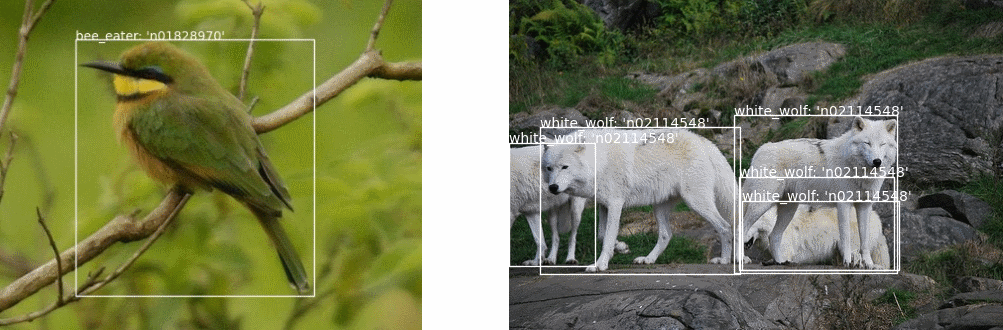
\includegraphics[scale=0.45]{annotation.png}
\caption{Collected ImageNet examples with annotations drawn.}
\label{dataimg}
\end{figure}

% caption PIL library was used

Much later into the project this script was upgraded to return the annotated image as a 2D array of 0's and 1's, with 1's inside the bounded regions to create a ground truth mask. The use of this mask for saliency calculation is described later (Section \ref{sec:metric}).

\section{Models \& Predictions} \label{sec:model}

Deep CNN models are expensive to train, so the high-level Keras library was used to import image classification models pre-trained on ImageNet \cite{keras}. Three models were chosen representative of common modern architectures (summarised in Table \ref{modeltable}). They acted as the underlying `black-box' models being explained.

\begin{table}[h]
\begin{tabular}{|l|l|l|l|}
\hline
\textbf{Model}       & \textbf{Structure}                                                                         & \multicolumn{1}{c|}{\textbf{Input Shape}} & \textbf{Project Role}  \\ \hline
\textbf{VGG16}       & \begin{tabular}[c]{@{}l@{}}16 stacked, 3x3 \\ convolutional layers\end{tabular}            & 224x224                                   & Most testing / results \\ \hline
\textbf{InceptionV3} & \begin{tabular}[c]{@{}l@{}}Stacked modules of \\ pooling + conv. layers\end{tabular}       & 299x299                                   & Supporting analysis    \\ \hline
\textbf{ResNet50}    & \begin{tabular}[c]{@{}l@{}}50-layer CNN with \\ `residual layer' connections.\end{tabular} & 224x224                                   & Supporting analysis    \\ \hline
\end{tabular}

\caption{Pre-trained image classifiers used in the project.}
\label{modeltable}
\end{table}

To check each model was working, a script was written to automate prediction collection and interact with preprocessed examples from the collected data. All software in the project was developed to be agnostic about the underlying model, though some methods required specific hyperparameters like a layer target. These targets were set up in a high level struct-type object in a constants file.

\section{Software Abstraction I}  \label{sec:sw1}

Each model requires input resizing and preprocessing in some form. An \textit{ImageHandler} class was therefore designed to abstract from complexity related to different representations of a single image instance. All input/output file methods and getter methods for raw, expanded and preprocessed representations were stored in this class, which made enforcing model agnosticity and method adaption later  (Section \ref{sec:adaption}) much easier.


\newpage
\section{Initial Method Investigation}  \label{sec:initial}

Public GitHub implementations for each of the four methods were downloaded: GradCAM \cite{gradcamrepo}, SHAP \cite{shaprepo}, DeepLIFT \cite{deepliftrepo} and LIME \cite{limerepo}.

They were then run on the VGG16 model. These out-of-the-box attributions are shown in Figure X.





\newpage
\section{Software Abstraction II}  \label{sec:sw2}

Siloed and overlapping logic for each method's implementation was cut out from the separate scripts for each method, and the common functions were extracted out into an \textit{Attributer} class fitted over the methods. 

Class Diagram


\newpage
\section{Adapting Methods for Compatibility}  \label{sec:adaption}

Some methods out-of-the-box were higher level implementations than others (SHAP and DeepLIFT). This made adaption more difficult, since they used their own representation form (e.g. heatmap) and internal methods that buried important functions like output normalisation.

\newpage
\section{Evaluation Metric Design} \label{sec:metric}

The motivation to create a new variant of an intersection-over-union metric, rather than rely on existing bounding box based comparison metrics, was based on observations in Related Work that existing metrics do not account for pixel-level detail and punish perforated saliency maps based on their reliance on a single component to find the box.

Performance wise, it is more taxing to account for pixel-wise attribution \textbf{cite?}.
\newpage
\section{Software Abstraction III}  \label{sec:sw2}


\newpage
\section{Result Collection}  \label{sec:result_collection}
GTX-1080.

\newpage
\section{Support for Other Models}



\end{document}